\section{am::lambda::binder\_\-const\_\-obj1$<$ R, P1, U, A1, A2 $>$ Struct Template Reference}
\label{structam_1_1lambda_1_1binder__const__obj1}\index{am::lambda::binder_const_obj1@{am::lambda::binder\_\-const\_\-obj1}}
{\tt \#include $<$lambda.hpp$>$}

Inherits {\bf am::lambda::detail::lambda\_\-op\_\-tag}.

Inheritance diagram for am::lambda::binder\_\-const\_\-obj1$<$ R, P1, U, A1, A2 $>$:\begin{figure}[H]
\begin{center}
\leavevmode
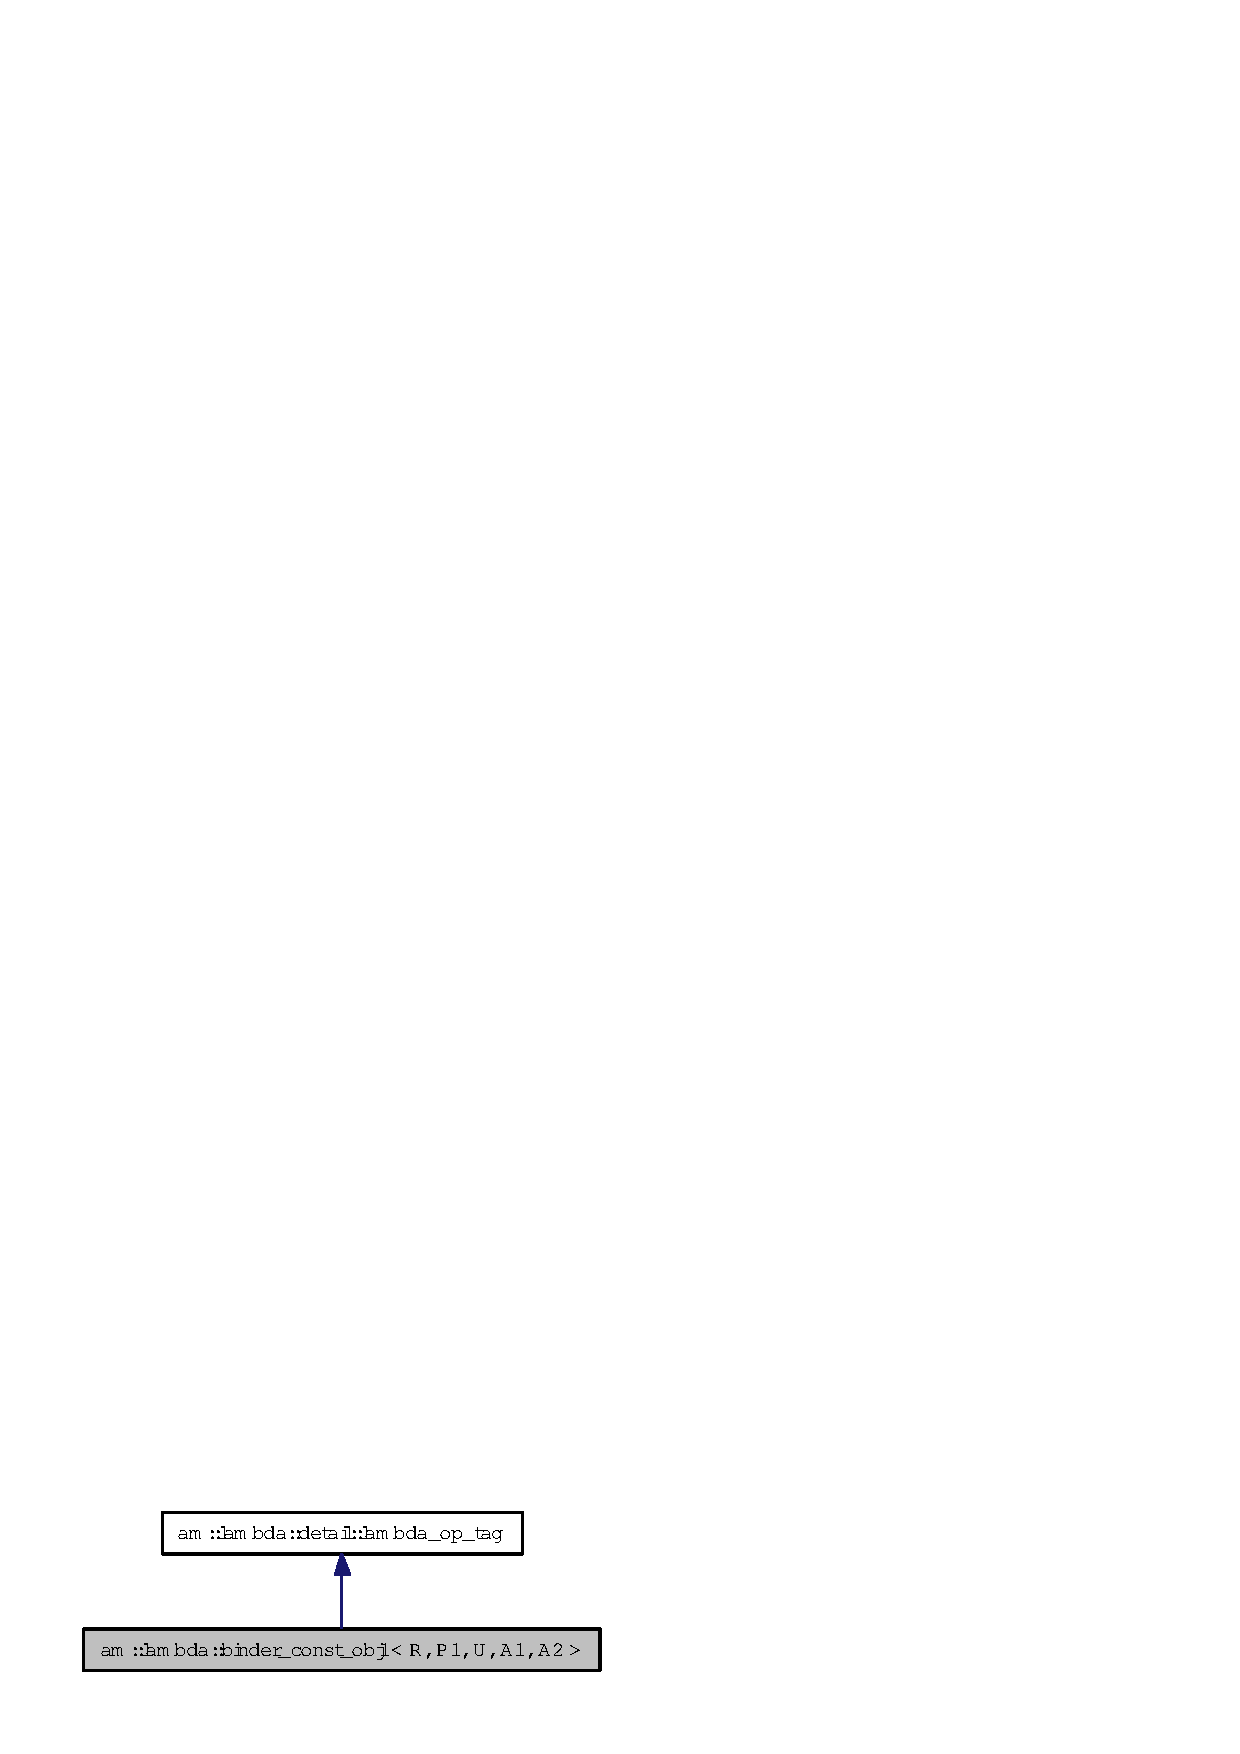
\includegraphics[width=146pt]{structam_1_1lambda_1_1binder__const__obj1__inherit__graph}
\end{center}
\end{figure}
Collaboration diagram for am::lambda::binder\_\-const\_\-obj1$<$ R, P1, U, A1, A2 $>$:\begin{figure}[H]
\begin{center}
\leavevmode
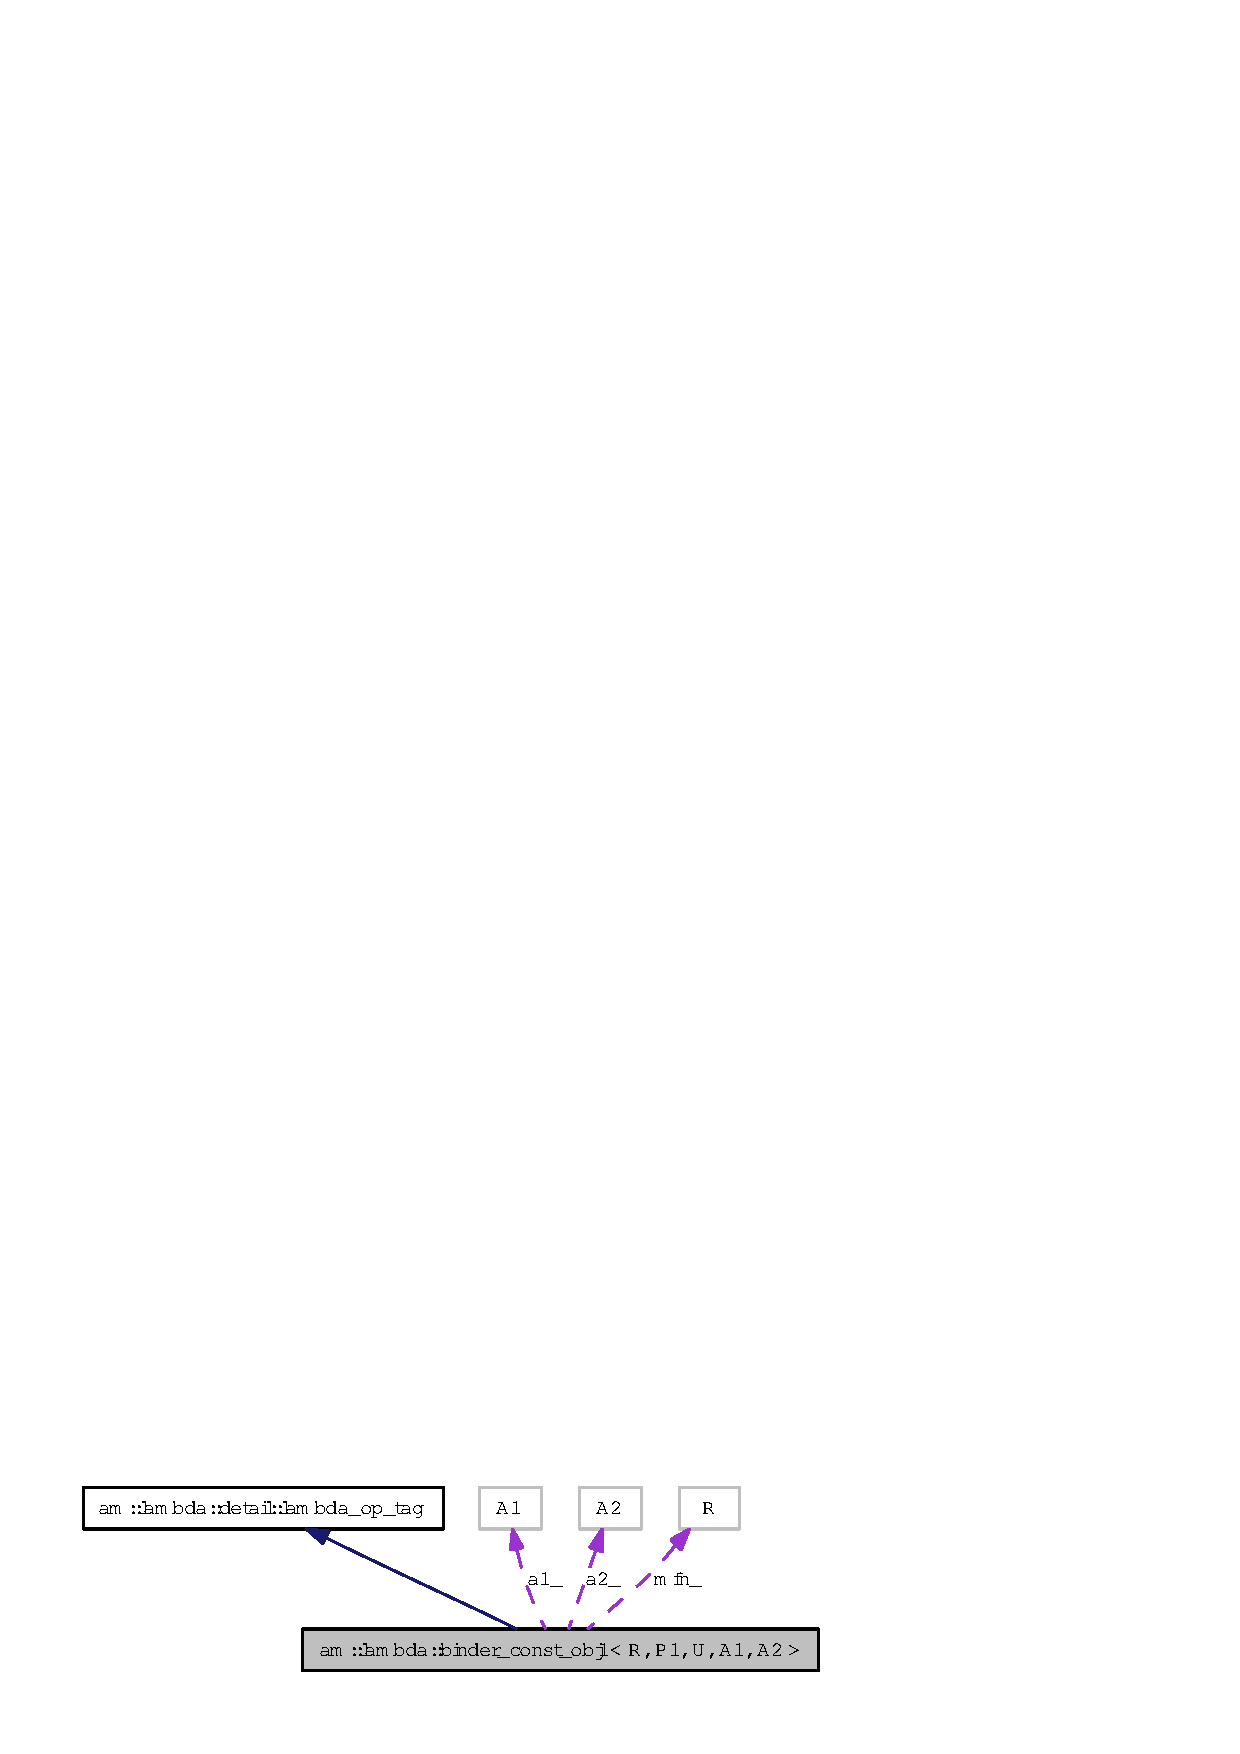
\includegraphics[width=198pt]{structam_1_1lambda_1_1binder__const__obj1__coll__graph}
\end{center}
\end{figure}
\subsection*{Public Types}
\begin{CompactItemize}
\item 
typedef detail::binder\_\-impl$<$ R $>$::result\_\-type \textbf{result\_\-type}\label{structam_1_1lambda_1_1binder__const__obj1_2e28710b27809b1164ec8049296c83b1}

\end{CompactItemize}
\subsection*{Public Member Functions}
\begin{CompactItemize}
\item 
\textbf{binder\_\-const\_\-obj1} (R(U::$\ast$mfn)(P1) const, A1 a1, A2 a2)\label{structam_1_1lambda_1_1binder__const__obj1_47feeaff4557f1447b3cdf4321e711d6}

\item 
template$<$class T1, class T2, class T3$>$ result\_\-type \textbf{operator()} (T1 t1, T2 t2, T3 t3) const \label{structam_1_1lambda_1_1binder__const__obj1_bdf91b1530eef1ae77363f1f0bf6611d}

\item 
template$<$class T1, class T2$>$ result\_\-type \textbf{operator()} (T1 t1, T2 t2) const\label{structam_1_1lambda_1_1binder__const__obj1_f956f6211d0e4b671a8da274fec1856b}

\item 
template$<$class T1$>$ result\_\-type \textbf{operator()} (T1 t1) const \label{structam_1_1lambda_1_1binder__const__obj1_d0454dd843d61eb2bd07ead76866e9ab}

\item 
result\_\-type \textbf{operator()} () const\label{structam_1_1lambda_1_1binder__const__obj1_04ad7a0a0b5403a039a855ef06daac01}

\end{CompactItemize}
\subsection*{Public Attributes}
\begin{CompactItemize}
\item 
R(U::$\ast$ \textbf{mfn\_\-} )(P1) const\label{structam_1_1lambda_1_1binder__const__obj1_ac9115fc1d2339910f7af5d3614b03f9}

\item 
A1 \textbf{a1\_\-}\label{structam_1_1lambda_1_1binder__const__obj1_fff32d21d2458b5c998e4c5e8ddc608d}

\item 
A2 \textbf{a2\_\-}\label{structam_1_1lambda_1_1binder__const__obj1_715b4504a65b59d36f9d2663a0f6d270}

\end{CompactItemize}


\subsection{Detailed Description}
\subsubsection*{template$<$typename R, typename P1, typename U, typename A1, typename A2$>$ struct am::lambda::binder\_\-const\_\-obj1$<$ R, P1, U, A1, A2 $>$}

Binder for the const member function which takes the first argument as object on which the member function is being called and one more argument. 



The documentation for this struct was generated from the following file:\begin{CompactItemize}
\item 
{\bf lambda.hpp}\end{CompactItemize}
